\documentclass{article}


\usepackage{circuitikz} %Für die Schaltpläne
\usepackage[T1]{fontenc}
\usepackage[utf8]{inputenc}
\usepackage{amsmath}
\usepackage{amssymb}
\usepackage{fancyhdr}
\usepackage{graphicx}
\usepackage{hyperref}
\usepackage{subcaption}
\usepackage{tikz}
\usepackage{cite}
\usepackage[nottoc, numbib]{tocbibind}
\usepackage{../assets/scripts/tex/color-env}
\usepackage[ngerman]{babel}



\usetikzlibrary{arrows}
\usetikzlibrary{arrows.meta,topaths}
\usetikzlibrary{bending}
\usetikzlibrary{calc}
\title{Elektrotechnik 1 Praktikum 1}


\usepackage[
includehead,
headheight = 17mm,
footskip = \dimexpr\headsep+\ht\strutbox\relax,
tmargin = 0mm,
bmargin = \dimexpr17mm+2\ht\strutbox\relax,
]{geometry}

\usepackage{anyfontsize}

\usepackage{xcolor}

\definecolor{DarkGreenBlue}{HTML}{264653}
\definecolor{LightGreenBlue}{HTML}{2A9D8F}
\definecolor{LightOrange}{HTML}{E9C46A}
\definecolor{DarkOrange}{HTML}{F4A261}
\definecolor{RedOrange}{HTML}{E76F51}
\definecolor{BrightRed}{HTML}{D62828}
\definecolor{DeepBlue}{HTML}{003049}



\pagestyle{fancy}
\fancyhead[L]{\leftmark}
\fancyhead[R]{}
\fancyfoot[L]{}
\fancyfoot[C]{\thepage}
\fancyfoot[R]{
\includegraphics[scale=0.2]{../assets/images/haw.jpg}}
\renewcommand\headrulewidth{0.5pt}


\begin{document}



\begin{tikzpicture}[overlay,remember picture]
  \thispagestyle{empty}
  \fill[black!2] (current page.south west) rectangle (current page.north east);

  \begin{scope}[transform canvas ={rotate around ={45:($(current page.north west)+(-.5,-6)$)}}]

    \shade[rounded corners=18pt, left color=DarkGreenBlue, right color=LightGreenBlue] ($(current page.north west)+(-.5,-6)$) rectangle ++(9,1.5);

  \end{scope}

  \begin{scope}[transform canvas ={rotate around ={45:($(current page.north west)+(.5,-10)$)}}]

    \shade[rounded corners=18pt, left color=LightOrange,right color=DarkOrange] ($(current page.north west)+(0.5,-10)$) rectangle ++(15,1.5);

  \end{scope}

  \begin{scope}[transform canvas ={rotate around ={45:($(current page.north west)+(0.5,-10)$)}}]

    \shade[rounded corners=8pt, right color=DarkOrange, left color=LightOrange] ($(current page.north west)+(1.5,-9.55)$) rectangle ++(7,.6);

  \end{scope}

  \begin{scope}[transform canvas ={rotate around ={45:($(current page.north)+(-1.5,-3)$)}}]

    \shade[rounded corners=12pt, left color=DeepBlue!80, right color=DeepBlue!60] ($(current page.north)+(-1.5,-3)$) rectangle ++(9,0.8);

  \end{scope}

  \begin{scope}[transform canvas ={rotate around ={45:($(current page.north)+(-3,-8)$)}}]

    \shade[rounded corners=28pt, left color=BrightRed, right color=BrightRed!80] ($(current page.north)+(-3,-8)$) rectangle ++(15,1.8);

  \end{scope}

  \begin{scope}[transform canvas ={rotate around ={45:($(current page.north west)+(4,-15.5)$)}}]

    \shade[rounded corners=25pt, left color=RedOrange, right color=DarkOrange] ($(current page.north west)+(4,-15.5)$) rectangle ++(30,1.8);

  \end{scope}

  \begin{scope}[transform canvas ={rotate around ={45:($(current page.north west)+(13,-10)$)}},]

    \shade[rounded corners=22pt, left color=DeepBlue,right color=DarkGreenBlue] ($(current page.north west)+(13,-10)$) rectangle ++(15,1.5);

  \end{scope}

  \begin{scope}[transform canvas ={rotate around ={45:($(current page.north west)+(18,-8)$)}},]

    \shade[rounded corners=8pt, left color=DarkOrange] ($(current page.north west)+(18,-8)$) rectangle ++(15,0.6);

  \end{scope}

  \begin{scope}[transform canvas ={rotate around ={45:($(current page.north west)+(19,-5.65)$)}},]

    \shade[rounded corners=12pt, left color=RedOrange] ($(current page.north west)+(19,-5.65)$) rectangle ++(15,0.8);

  \end{scope}

  \begin{scope}[transform canvas ={rotate around ={45:($(current page.north west)+(20,-9)$)}}]

    \shade[rounded corners=20pt, left color=BrightRed, right color=BrightRed!80] ($(current page.north west)+(20,-9)$) rectangle ++(14,1.2);

  \end{scope}

  \draw[ultra thick,gray] ($(current page.center)+(5,2)$) -- ++(0,-3cm) node[midway,left=0.25cm,text width=5cm,align=right,black!75]{{\fontsize{25}{30} \selectfont \bf Elektronik 2\\[10pt] Praktikum 4}} node[midway,right=0.25cm,text width=6cm,align=left,orange]{{\fontsize{70}{86} \selectfont 2021}};

  \node at ($(current page.center)+(0,-4)$) {{\fontsize{60}{72} \selectfont Leistungsverstärker}};

  \node[text width=8cm,align=center] at ($(current page.center)+(0,-6.5)$) {{\fontsize{16}{20} \selectfont \textcolor{orange}{ \bf \today}} \\[3pt] Florian Tietjen\\[3pt] Torsten Möller\\[3pt] Eric Antosch};

\end{tikzpicture}
\newpage
\thispagestyle{empty}

\tableofcontents

\listoffigures
\listoftables
\newpage

\section{Einleitung}
\label{sec:einleitung}

In diesem Laborversuch wollen wir uns mit der Wirkweise und den Eigenschaften eines Leistungsverstärkers auf der Basis eines Operationverstärkers (OPA551) beschäftigen. Die Inbetriebnahme, die Übernahmeverzerrung, Leistungsaufnahme und der Klirrfaktor sind dabei Gegenstand der Überlegungen und Untersuchungen.

\section{Inbetriebnahme}
\label{sec:inbetriebnahme}

\begin{task}
  TIn der ersten Aufgabe wollen wir den Leistungsverstärker in Betrieb nehmen. Dazu wählen wir die Schalterstellung B (siehe \ref{fig:schalt1}) und drehen die Strombegrenzung stark zurück, sodass die Ruhestromaufnahme nur einige mA beträgt. Wir vergrößern langsam die Strombegrenzung auf 80\% und speisen ein Eingangssignal von $U_{e} = 0,1V$ mit $f = 1kHz$ ein. Am $R_{L}$ sollte eine Spannung von $1V$ erscheinen.
\end{task}

\begin{figure}[h]
  \centering
  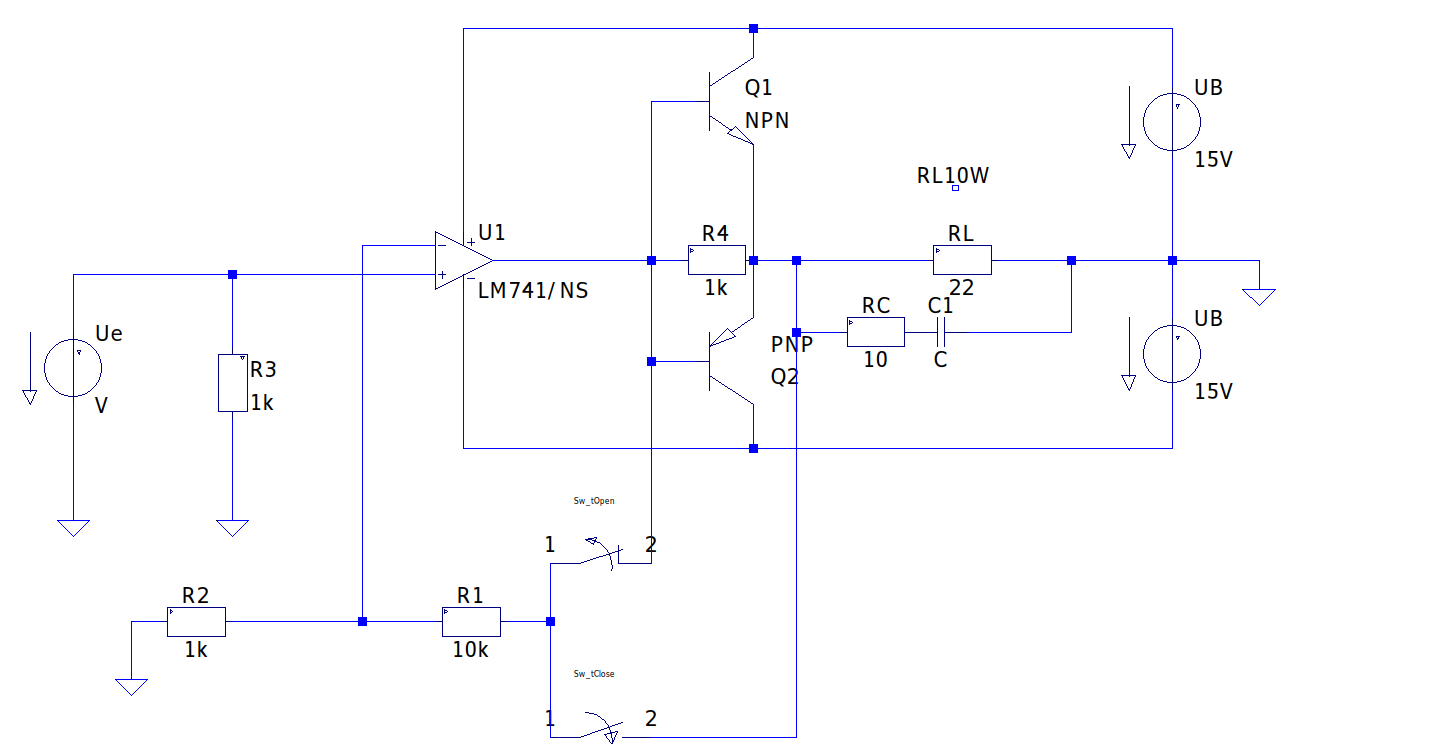
\includegraphics[width=\textwidth]{../assets/images/ELP2_4/schalt1.png}
  \caption{Grundschaltung des Leistungsverstärkers}
  \label{fig:schalt1}
\end{figure}

\subsection{Vorbereitung}
\label{sec:vorbereitung}

Wir wollen zudem erst einmal die theoretische Verstärkung des Leistungsverstärkers berechnen. Dafür machen wir uns bewusst, dass es sich hier um eine rückgekoppelte nicht-invertierende Verstärkerschaltung handelt. Es folgt:

\begin{equation}
  \label{eq:1}
  A_{u} = \frac{R_{1}+R_{2}}{R_{2}} = \frac{10k\Omega + 1k\Omega}{1k\Omega} = 11
\end{equation}

Wir erwarten daher eine Verstärkung von $U_{e} = 0,1V$ zu $U_{a} = A_{u} \cdot U_{e} = 11 \cdot 0,1V = 1,1V$.

\subsection{Duchführung}
\label{sec:duchfuhrung}

Wir stellen eine Betriebsspannung von $U_{B} = 15V$ ein und stellen die Stromverstärkung vollständig zurück. Wir regen den Eingang mit einem sinusförmigen Signal $U_{e} = 0,1V$ an und die Stormbegrenzung wird nun langsam auf 80\% erhöht. Wir messen sowohl das Eingangs -und Ausgangssignal auf dem Oszilloskop.

\begin{figure}[h]
  \centering

  \caption{Messung der Inbetriebnahme}
  \label{fig:osziinbetrieb}
\end{figure}

Wir erkennen nun, dass wir mit

\begin{equation*}
  A_{u} = \frac{U_{a}}{U_{e}} = \frac{1,04V}{91,2mV} = 11,04
\end{equation*}

eine sehr ähnliche Verstärkung erhalten, wie wir zuerst theoretisch betrachtet hatten.

\subsection{Auswertung}
\label{sec:auswertung}

Die Abweichung lässt sich auf die Bauteile und das Oszilloskop zurückführen. Dort können parasitäre Effekte der Leitungen, korrodierte Kontakte oder ähnliche Umstände einen Einfluss auf das Ergebnis nehmen.

\newpage
\section{Übertragungskennline Ua=f(Ue), Übernahmeverzerrung}
\label{sec:ubertr-ua=f-ubern}

\begin{task}
  TIn nächsten Schritt wollen wir uns nun auf die Übernahmeverzerrung der Schaltung beziehen. Dazu messen wir sowohl bei Schalterstellung A als auch bei Schalterstellung B mithilfe des X-Y-Betriebs des Oszilloskops die Ausgangsspannung in Abhängigkeit von der Eingangsspannung. Der bereich der Ausgangsspannung liegt dabei bei ca. $\pm 1V$.
\end{task}

\subsection{Vorbereitung}
\label{sec:vorbereitung-1}

Durch die in der Schaltung verbauten Transistoren und den Operationsverstärker werden beide Halbwellen des sinusförmigen Eingangssignals verstärkt. Für die Schalterstellung A gilt, dass die Rückkopplung vor der Gegentakt-Endstufe mit $U_{BE} = 0,6V$, $A_{u} = 11$, $U_{a,op} = U_{e} \cdot A_{u} = U_{e} \cdot 11 \implies U_{a} = U_{a,op} - U_{BE}$. Daraus folgt dann, dass $U_{a} = U_{e} \cdot A_{u} - U_{BE} = 0,1V \cdot 11 - 0,6V = 0,5V$ (bei maximaler Verstärkung). Wir wollen nun noch heraus finden, in welchem Bereich eine Ausgangsspannung messbar ist. Dazu wissen wir, dass für die positive Halbwelle gilt $U_{a,op} \geq U_{BE}$. Daraus folgt:
\begin{equation*}
  min(U_{e}) = \frac{min(U_{a,op})}{A_{u}} = \frac{U_{BE}}{A_{u}} = \frac{0,6V}{11} = 55mV
\end{equation*}
Analog zu dieser Überlegung ergibt sich, dass die negative Halbwelle für einen Wert von bis zu $-55mV$ keine Ausgangsspannung liefert, da dort die Endtransistoren noch nicht durchsteuern.\\
Für die Schalterstellung B ist wie in Aufgabe 1 folgende Überlegung
\begin{equation*}
  U_{a,op} = U_{a} = U_{e} \cdot A_{u} = 0,1V \cdot 11 = 1,1V
\end{equation*}

Es ist also zu erwarten, dass bei der Schalterstellung A die Lissajous-Figur einen Bereich hat ($55mV-(-55mV)$), indem keine Y-Ablenkung auf das Signal von dem Kanal 1 zu erkennen ist. Wir erwarten bei Schalterstellung B eine durchgehende Linie, also ein Frequenzverhältnis von 1:1 und keine Phasenverschiebung.

\subsection{Duchführung}
\label{sec:duchfuhrung-1}

Wir wollen zuerst die Signale, also das Ein -und Ausgangssignal mithilfe des Y-T-Betriebs sauber einstellen und dann im X-Y-Betrieb eine entsprechende Darstellung dokumentieren.

\begin{figure}[h]
  \centering

  \caption{Messung der Schalterstellung A}
  \label{fig:schaltAlissa}
\end{figure}

\begin{figure}[h]
  \centering

  \caption{Messung der Schalterstellung B}
  \label{fig:schaltBlissa}
\end{figure}

\subsection{Auswertung}
\label{sec:auswertung-1}

Schalterstellung A

Schalterstellung B



\section{Aufgenommene Leistung, Ausgangsleistung, Verlustleistung}
\label{sec:aufg-leist-ausg}

\begin{task}
  TWir wollen nun als nächstes die Leistung unserer Schaltung untersuchen. Mit einer Schalterstellung B, $f=1kHz$ und einer Strombegrenzung von 100\% messen wir die Ausgangsspannung $U_{a}$ und die Kollektorströme $I_{C1}$ und $I_{C2}$ für einen Eingangssignalbereich von $U_{e} = 0...0,5V$ dar. Im Anschluss wollen wir die Ausgangsleistung $P_{A}$, die aufgenommene Leistung der Endstufe $P_{B}$, die Verlustleistung der Endstufe $P_{V}$ und den Wirkungsgrad der Endstufe $\eta$ in Abhängigkeit von der Eingangsspannung grafisch darstellen.
\end{task}

\subsection{Vorbereitung}
\label{sec:vorbereitung-2}

Wir berechnen die Werte $P_{A}$, $P_{B}$, $P_{V}$ und $\eta$ wie in der Vorlesung angegeben:

\begin{align*}
  P_{A} &= \frac{U_{A}^{2}}{R_{L}}\\
  P_{B} &= (i_{C2} + i_{C1})\cdot U_{B}\\
  P_{V} &= P_{B} - P_{A}\\
  \eta &= \frac{P_{A}}{P_{B}}\\
\end{align*}

Wir erwarten dabei die in der Vorlesung erklärten Graphen:

\begin{figure}[h]
  \centering

  \caption{Erwartungen von den zu untersuchenden Werten aus der Vorlesung}
  \label{fig:erwartung}
\end{figure}

\subsection{Durchführung}
\label{sec:durchfuhrung}

\begin{table}[h]
  \centering
  \begin{tabular}{|c|c|c|c|c|c|c|c|}
    $U_{e}$& $U_{a}$ & $I_{C1}$& $I_{C2}$&$P_{A}$&$P_{B}$&$P_{V}$& $\eta$\\
    \hline
  \end{tabular}
  \caption{Messergebnisse der zu untersuchenden Werte}
  \label{tab:messungauf3}
\end{table}

Aus den Messergebnissen können wir folgende Graphen plotten:


\begin{figure}[h]
  \centering

  \caption{Plot der Leistungen}
  \label{fig:powerplot}
\end{figure}


\begin{figure}[h]
  \centering

  \caption{Plot des Wirkungsgrades}
  \label{fig:eff}
\end{figure}

\subsection{Auswertung}
\label{sec:auswertung-2}



\bibliographystyle{plain}
\bibliography{ELP2_1}{}
\end{document}
